\documentclass{article}
\usepackage{xr}
\usepackage{lscape}

\usepackage{graphicx}
\usepackage{authblk}
\usepackage{amsfonts}
\usepackage{pifont}

\renewcommand{\tablename}{Supplementary Table}
\renewcommand{\figurename}{Supplementary Figure}
\newcommand{\rowgroup}[1]{\hspace{-1em}#1}


\begin{document}


\title{Eagle makes multi-locus association mapping on a genome-wide scale routine}
\author[1]{Andrew W. George}
\author[1]{Arunas Verbyla}
\author[2]{Joshua Bowden}

\affil[1]{Data61, CSIRO, Australia.}
\affil[2]{IM \&T, CSIRO, Australia.}

\maketitle






\begin{landscape}

\begin{table}
\caption{Implementation and methodology attributes of eight computer programs/packages for genome-wide association mapping.  }
\label{suptabsummary}
\vspace{0.5cm}
\begin{tabular}{lcccccccc} \hline
                                                   Attributes                  & {\bf Eagle}                                 & {\bf bigRR}             & {\bf glmnet}            & {\bf LMM-Lasso}                    & {\bf MLMM} & {\bf r2VIM}      & {\bf FaST-LMM} & {\bf GEMMA} \\  \hline
{\bf {\em Implementation}}    &         &            &             &                   &            &                &      &      \\ [0.15cm]
\hspace{1mm}  Purpose built$^a$    &   Yes     &    Yes      &  No   &   Yes  &  Yes  &  Yes  & Yes  & Yes          \\ [0.15cm]


\hspace{1mm}  Language                 &  R/C++       &    R        &      R       &     Python     &  R          &    R         &  C++ and     &   C++   \\  
                                                          &         &            &             &                   &            &                                     &   Python$^b$       &      \\  [0.15cm]

\hspace{1mm} GUI                            & Yes &    No      & No          &  No    &  No    &   No     & No     & No    \\  [0.15cm]




\hspace{1mm} Documentation        &  Videos,  user-manuals,              &    R help       &  Vignettes,    &   Readme.txt,       &   Vignette,          &     R help           &   Videos, website             &  User-manual,     \\  
                                                        &  website,    R help     &                      &  R help         &    test script           &  R help              &                           &    user-manuals,  &   website  \\ [0.15cm]
                                                                                         
\hspace{1mm} Additional fixed        &   Yes   &      Yes      &     Yes    &  No                 &      Yes      &      No          &      Yes & Yes     \\  
\hspace{1mm} effects$^c$               &           &                   &                 &                   &                   &                     &              &      \\  [0.15cm]

\hspace{1mm} Types of  &  Cont.      &   Cont.,          &   Cont.,           &   Cont.                 &   Cont.          &     Cont.,          &   Cont.   &  Cont.,    \\  
\hspace{1mm} trait data  &                &    binary,      &      binary,         &                   &            &     binary           &      &   binary    \\  
                                      &                &   count         &       count          &                   &            &                &      &      \\  [0.15cm]


\hspace{1mm} Data larger                   &   Yes    &      No      & No          &  No    &  No    &   No     & Yes      & No    \\  
\hspace{1mm} than memory                                             &         &            &             &                   &            &                &      &      \\  [0.8cm]


{\bf {\em Methodology} }   &         &            &             &                   &            &                &      &      \\  [0.15cm]
\hspace{1mm}  Model $^d$                    & LMM   & HEM  &  GLMM &   LMM  & LMM  & RF & LMM   & LMM, mvLMM\\ 
                      					    &             &   &              &             &          &        &           &   Bayesian Sparse LMM      \\  [0.15cm]
					    
\hspace{1mm} SNPs fitted $^e$      &    All/multiple      &    All       &   All        &      All          &  Multiple          &  Multiple              &   Single   &  Single   \\  [0.15cm]


\hspace{1mm}  Selection type             & Model   & Variable  &  Variable &  Variable  &  Model  &  Variable & Variable  & Variable \\  [0.15cm]

\hspace{1mm} Threshold free      &    Yes     &  No    &  No         &    No               &     Yes       &  No              &  No   & No      \\  [0.15cm]  \hline
           

\end{tabular}
{$^a$ \scriptsize{Specifically created for the analysis of GWAS data.}}\\
{$^b$ \scriptsize{Separate programs, one written in Python, the other C++}} \\
{$^c$ \scriptsize{Capacity for additional fixed effects (such as  age, sex, and/or population structure effects) to be included directly in the model.}} \\
{$^d$ \scriptsize{For the different types of model, 
LMM is linear mixed model.  GLM is generalised linear model., GLMM is generalised linear mixed model, and RF is random forests.}} \\
{$^e$ \scriptsize{Association is assessed a SNP at a time (single), for multiple SNPs (multiple), or for all SNPs (all). Eagle fits all SNPs but also identifies multiple SNPs (All/multiple) in association with the trait.} } \\
\end{table}


\end{landscape}






\begin{figure}
\caption{Power verse false discovery rates for Eagle and the multi-locus methods. Plots for only those simulation 
scenarios where all multi-locus methods could be implemented are shown.  Eagle has the highest power across the four 
scenarios but MLMM also performs well. A false discovery rate of greater than 10\% is typically not employed in GWASs so the 
upper limit of the x-axis is 0.1.}
\label{supfigpowermultiple}
\begin{center}
\includegraphics[width=15cm, height=15cm]{power1main.eps}
\end{center}

\end{figure}





\begin{figure}
\caption{Memory usage (in gigabytes) of Eagle and the other association mapping programs/packages across 
the six simulation scenarios. The maximum amount of memory on the computer is 128 gigabytes. 
The x-axis is on the log scale. GEMMA, a single-locus implementation, had the lowest memory usage. 
Of the multi-locus implementations, Eagle had the lowest memory usage. Also, it 
was the only multi-locus 
implementation able to produce results for data under  scenario 10000 x 1.5M. This is due to its ability 
to handle data larger than the available memory of a computer. FaST-LMM was run where all the SNP data are used 
to estimate the relationship matrix (FaST-LMM$^{all}$)   and where genotype data from every five-hundredth SNP are used to 
estimate the relationship matrix (FaST-LMM$^{few}$)}.
\label{supfigmem}

\begin{center}
\includegraphics[width=15cm, height=15cm]{mem.eps}
\end{center}
\end{figure}






\begin{table}[h]
\scriptsize
\caption{New SNP-trait associations found from the analysis of the mouse data with Eagle.  Due to many of the traits in the study 
being correlated, genetically,  these new findings could be confirmed through their prior discovery with other traits in the original 
mouse study (Prior Associations). }
\label{suptabnew}
\vspace{0.5cm}
\begin{tabular}{lcccp{6cm}}  \hline
     & \multicolumn{3}{c}{New SNP-trait Association}  &  \\  \cline{2-4}
Method           &  Trait  & Chrm  &  Position (Mb)  & \hfil Prior Associations  \\  \hline  
Eagle$^{alt}$  & Bioch.HDL   & 6   & 17.53         & Muscles.Sol.g Muscles.TA.g Muscles.Plant.g Muscles.EDL.g  Muscles.Gast.g 
     SPPI.ln.pa Bioch.Calcium    Bioch.Tot.Cholesterol Bioch.Tot.Protein Bioch.Albumin \\ 
                       & Bioch.LDL   & 6    &  17.53        & Muscles.Sol.g Muscles.TA.g Muscles.Plant.g Muscles.EDL.g  Muscles.Gast.g SPPI.ln.pa Bioch.Calcium  Bioch.Tot.Cholesterol Bioch.Tot.Protein Bioch.Albumin \\  
 Eagle$^{optimal}$  &        Bioch.Tot.Cholesterol  & 4      &  134.58  & FACS.CD3posCD44posCD4CD8Ratio  \\
                        & Bioch.HDL                  & 4      &  134.58  & FACS.CD3posCD44posCD4CD8Ratio   \\
                        &                                    & 6      &    17.53   & Muscles.Sol.g Muscles.TA.g Muscles.Plant.g Muscles.EDL.g  Muscles.Gast.g 
     SPPI.ln.pa Bioch.Calcium    Bioch.Tot.Cholesterol Bioch.Tot.Protein Bioch.Albumin  \\
                        & BMC.Mean                 & 15    &     86.57  & BMC.Median \\
                        & BMC.Mean.N             &  5     &     24.64   &  BMC.Mean BMC.StdDev BMC.StdDev.N  BMC.Max.N  BMC.Median BMC.Kurt
                        BMC.Max BMC.Kurt.N  \\
                        & BMC.Max.N               & 15    &      86.57  & BMC.Median \\
                        & Bioch.LDL                  & 6      &   17.53   & Muscles.Sol.g Muscles.TA.g Muscles.Plant.g Muscles.EDL.g  Muscles.Gast.g 
     SPPI.ln.pa Bioch.Calcium    Bioch.Tot.Cholesterol Bioch.Tot.Protein Bioch.Albumin  \\  \hline
                                           
                       
                    

\end{tabular}
\end{table}


%% This table appears in Figure 1 in paper. It's included here in case I need to regenerate the table. 
%%
%%\begin{table}
%%\caption{The median run times (in minutes) of Eagle and the other association mapping programs across the six simulation scenarios. }
%%\begin{tabular}{llcccccc}
%%              &           &  \multicolumn{6}{c}{Simulation Scenarios} \\ \cline{3-8}
%% Method & Name & 150 x 5K & 1500 x 50K & 350 x 400K & 2000 x 500K & 4000 x 1.5M & 10000 x 1.5M \\ \hline
%% Multiple & Eagle 	&	   0.08  &   1.62   &  \bf{2.7}1  &   \bf{13.65}   & \bf{127.63}  &   699.55  \\
%%               & MLMM 	&	   0.15    &  2.91    & 19.04  &  143.01  &  870.84  &     \\
%%              & glmnet 	&	  0.11     & 3.95    & 14.06    & 74.03    &        &    \\
%%               & r2VIM 	&	   0.09    &  3.66    &  5.51    & 50.59    & 380.52  &   \\ 
%%               & bigRR 	&	    1.01   & 113.35   &  54.99   & 1030.61  &        &     \\
%%               & LMM-Lasso 	&     0.57  &   52.08 &    92.20  & 1031.85 &           &     \\ \\
%%Single     &  GEMMA 	&      0.02  &   5.02   &   6.17  &   84.83   & 723.33  & 4071.60 \\
%%               & FaST-LMM$^{few}$ 	&    \bf{0.01}   &  \bf{0.80}   &   7.07   &  20.16   & 193.90   & \bf{346.19} \\ 
%%               & FaST-LMM$^{all}$   	&   0.03   & 2.96  &    7.90   &  41.27  &            &   \\ \hline
%%\end{tabular}
%%
%%\end{table}







\end{document}
